% Created 2021-03-13 Sat 23:10
% Intended LaTeX compiler: pdflatex
\documentclass[11pt]{article}
\usepackage[utf8]{inputenc}
\usepackage[T1]{fontenc}
\usepackage{graphicx}
\usepackage{grffile}
\usepackage{longtable}
\usepackage{wrapfig}
\usepackage{rotating}
\usepackage[normalem]{ulem}
\usepackage{amsmath}
\usepackage{textcomp}
\usepackage{amssymb}
\usepackage{capt-of}
\usepackage{hyperref}
\usepackage[spanish]{babel}
\usepackage[margin=1.5cm]{geometry}
\usepackage{arev}
\author{Edgar Quiroz}
\date{\today}
\title{Serpientes y Escaleras a distancia\\\medskip
\large Versión de sólo texto para Google Meet}
\hypersetup{
 pdfauthor={Edgar Quiroz},
 pdftitle={Serpientes y Escaleras a distancia},
 pdfkeywords={},
 pdfsubject={},
 pdfcreator={Emacs 27.1 (Org mode 9.5)}, 
 pdflang={Spanish}}
\begin{document}

\maketitle

\section{Planteamiento}
\label{sec:orgdbba6c4}

El objetivo es comprobar la necesidad de adaptar las reglas cuando el medio
cambia. Deberán crear reglas adaptadas para jugar el juego de mesa de Serpientes
y Escaleras, suponiendo que se va a jugar vía videoconferencia y la mayoría de
los participantes por problema de conectividad no pueden prender su cámara ni su
micrófono.

La tarea debe ser un corto documento que incluya el nombre del alumno, las
reglas adaptadas y las observaciones que consideren necesarias de su adaptación
(que no se puede realizar, que sí o porque de cierta adaptación especial)

\section{Reglas tradicionales}
\label{sec:orgceb3c79}

Normalmente se tiene un tablero rectangular con casillas numeradas desde el 1.
Algunas casilla están conectadas por serpientes o escaleras, de tal forma que
la boca de las serpientes siempre está en una casilla superior y la base de las
escaleras siempre está en una casilla inferior. Estás tienen el siguiente
funcionamiento

\begin{itemize}
\item Al caer en la boca de una serpiente hay que moverse a la cola de la serpiente
\item Al caer en la base de una escalera hay que moverse a la cima de la escalera.
\end{itemize}

Además, si se se lanza el dado y se requiere mover a casillas más allá de la
última, se debe recorrer las casillas extra en sentido inverso. La manera de
moverse está resumida en la figura \ref{fig:move-flux}.

\begin{figure}[htbp]
\centering
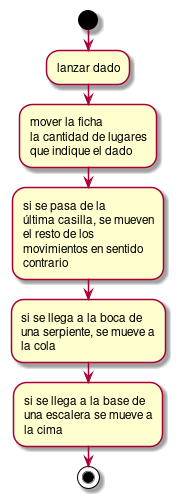
\includegraphics[scale=0.75]{imgs/move_flux.png}
\caption{\label{fig:move-flux}Pasos para moverse en una jugada.}
\end{figure}

Para jugar además se necesitan al menos dos jugadores, un dado, una ficha por
jugador y definir un orden para jugar. Al inicio del juego todos los jugadores
colocan su ficha en la primera casilla. Cada vez que sea su turno deben

\begin{itemize}
\item Lanzar el dado
\item Mover su ficha como se indicó anteriormente
\item Si se llega a la última casilla, gana.
\end{itemize}

Cuando gané la primera persona se detiene el juego. El resumen de estas reglas
se puede ver en la figura \ref{fig:normal-flux}.

\begin{figure}[htbp]
\centering
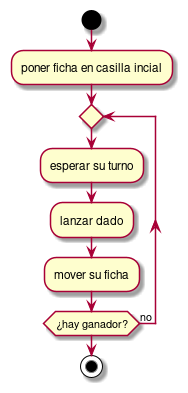
\includegraphics[scale=0.75]{imgs/normal_flux.png}
\caption{\label{fig:normal-flux}Flujo normal del juego}
\end{figure}

\section{Reglas modificadas}
\label{sec:org86edfd7}

Al no tener acceso a un tablero común para ver las posiciones de los demás, en
esta versión se va a considerar un encargado para llevar registro de estos
datos. Se le denomina \guillemotleft{}moderador\guillemotright{}.

\subsection{Moderador}
\label{sec:org1ef8bcf}

El moderador será el encargado de tener registro de lo que normalmente se
tendría en un tablero. Así que antes del juego debe

\begin{itemize}
\item Decidir el tablero
\item Tener un espacio para registrar a los jugadores y su posición actual
\item Tener algún tipo de dado
\end{itemize}

Al iniciar el juego debe

\begin{itemize}
\item Anotar a los jugadores.
\item Indicar la posición de las serpientes y escaleras en el tablero.
\end{itemize}

El orden en que se anoten será el orden en el que jugarán. Durante el juego se
debe

\begin{itemize}
\item Indicar a los jugadores cuando sea su turno
\item Esperar una confirmación de ellos
\item Tirar el dado y anunciar el resultado
\item Mover al jugador siguiendo las reglas normales
\item Indicar si se llegó a una serpiente, escalera o si ganó.
\item Anunciar la posición final del jugador.
\end{itemize}

Se repetirá esto hasta que un jugador llegue a la casilla final. Entonces se
anuncia al ganador y se termina el juego. El resumen de las acciones del
moderador se puede ver en el la figura \ref{fig:mod-flux}.

\begin{figure}[htbp]
\centering
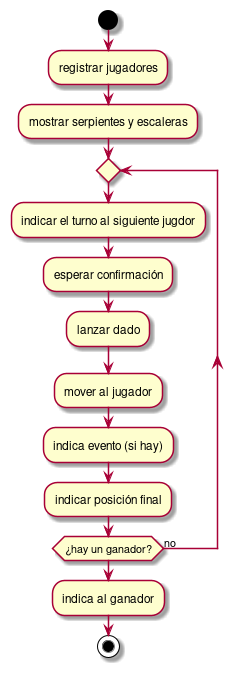
\includegraphics[scale=0.75]{imgs/moderador_flux.png}
\caption{\label{fig:mod-flux}Flujo de actividades para el moderador}
\end{figure}

\subsection{Jugador}
\label{sec:orgd1140fc}

Como la mayor parte del trabajo la realiza el moderador, los jugadores
simplemente tienen que indicar que quiere jugar, y luego esperar que el
moderador les pida confirmar su turno. Este flujo se puede ver en la figura
\ref{fig:player-flux}.

\begin{figure}[htbp]
\centering
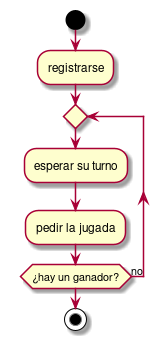
\includegraphics[scale=0.75]{imgs/player_flux.png}
\caption{\label{fig:player-flux}Flujo para el jugador}
\end{figure}
\end{document}
